\chapter{Basic colour strategy}
\label{s:basic-operators}

\setcounter{figure}{1}

To complete the definition of the basic colour strategy, I need
to introduce its adoption, alignment and invention operator. The
invention operator allows users to expand the current language system
whenever they feel it is insufficient for their communicative
needs. This expansion involves the invention of a new colour category
and a lexical rule to express this category in language. The adoption
operator allows language users to pick up these newly invented terms
and the corresponding colour categories. The alignment operator
specifies how language users can align their linguistic knowledge both
on the syntactic and the semantic level.

\section{Related models}

In \chapref{s:basic-strategy}, I already introduced various models
\citep{steels05coordinating, belpaeme05explaining, belpaeme07language,
  puglisi08cultural, baronchelli10modeling} that adhere to the
language game paradigm and use the colour naming game. The goal of
these studies was to study how a population of agents could coordinate
their own colour category system through local interactions.

Other models for the coordination of a colour category system have
been proposed as well. One model is more in line with the iterated
learning model \citep{smith03iterated} in which the burden of the
explanation is placed on the idea that a language learner will have to
generalise from only a limited number of observations instead of the
communicative function. In this model, colour categories are inferred
using Bayesian inference and invention is based on a random choice
\citep{dowman07explaining}.

Another mathematical model focusses on a discrimination task for which
the expected outcome depends on the similarity of the colours that
need to be discriminated. In this model, a circular conceptual colour
space is deployed, in which any typology of categories is as likely to
occur as others. Adding heterogeneity to the model, either in the
population or in the likelihood that a particular colour is presented
to the agents or both, breaks this symmetry
\citep{komarova08population}.

\section{Adoption and alignment operators}
\label{s:bcs-adoption-alignment-operators}

The main goal of the adoption and alignment operators is to ensure
that one agent can acquire the language system of another agent. It
needs to learn the private knowledge of the language system that is
being used in such a way that is sufficiently coordinated to ensure
communicative success.

The adoption operator\is{learning operators!adoption operator!for basic colour strategy}
is used to learn the colour categories of
another agent that are unknown to the learning agent. The main trigger
for this operator is hearing an unknown colour term. The application
of this operator results in learning a new category that is focussed
on the colour of the topic of the current interaction. The unknown
colour term is associated with this new category. This operator is in
line with research in developmental psychology which showed the
influence of learning a category upon hearing a new label
\citep{xu02role}. Note that this implementation of the adoption
operator implies that no synonyms will be present in the resulting
language system.

The alignment operator\is{learning operators!alignment operator!for
  basic colour strategy} is implemented by shifting the prototype of
the category that was used in the direction of the colour of the
topic. It is used by both speaker and hearer after a successful
interaction. The rate by which this shift happens is controlled by
\textsc{colour category alignment rate} 
\is{alignment rate!colour category} 
\is{colour category alignment rate|see{alignment rate}} 
($r_a$) which linearly specifies the new
location of the prototype ($c_{n+1}$) on the line segment between the
old location of the prototype ($c_n$) and the topic ($t$). The exact
formula is shown in Equation \ref{eq:alignment_rate}. If the alignment
rate is 0, the prototype does not shift at all, whereas at a rate of
1, the new location would be the topic of the last interaction. In all
experiments reported in this book, the alignment rate is fixed to
0.05, unless stated otherwise. An illustration of an alignment rate is
given in \figref{f:alignment-rate}.

\begin{equation}
c_{n+1} = (1 - r_a) c_n  + r_a t
\label{eq:alignment_rate}
\end{equation}

\begin{figure}[htbp]
  \begin{center}
    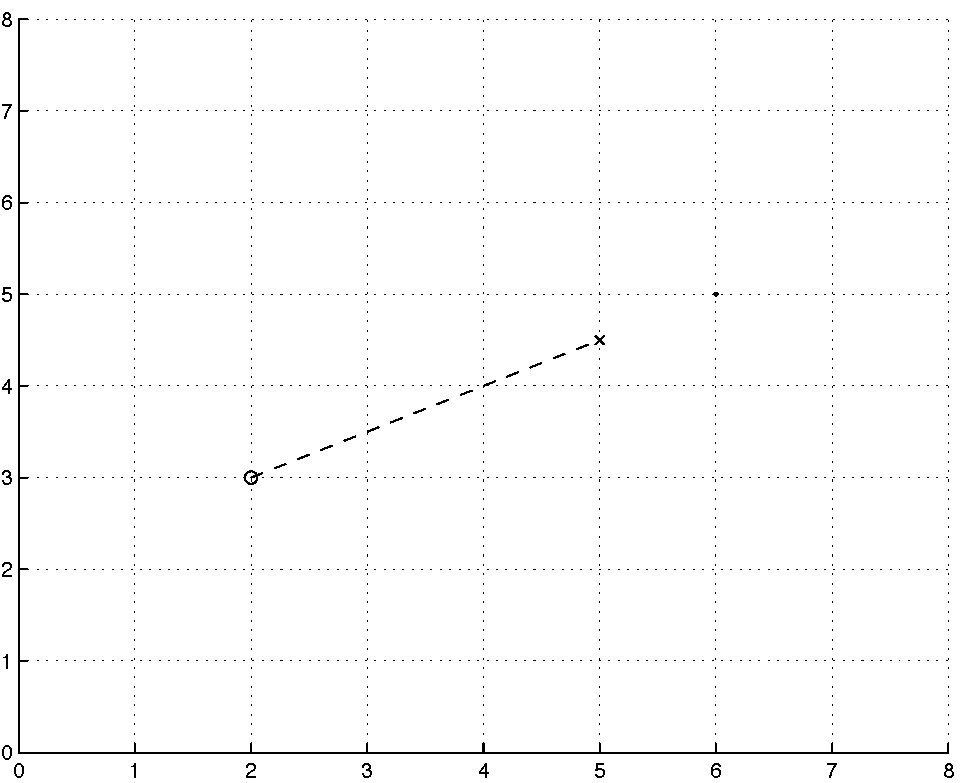
\includegraphics[width=.55\textwidth]{./basic-operators/figures/alignment-rate.pdf}
    \caption[Illustration of the alignment rate]{Illustration of the
      alignment rate. Before the game, the prototype of the category
      was at (2,3). The colour of the topic sample was located at
      (6,5). Given that the interaction was successful and the
      alignment rate is 0.75, the location of the prototype will
      become (5,4.5).}
    \label{f:alignment-rate}
  \end{center}
\end{figure}

\subsection{Acquisition experiment}
\is{acquisition experiment!for basic colours strategy}

In the acquisition experiment, one agent needs to acquire the language
system known by another agent. This will allow me to assess the
effectiveness of the acquisition operators. The language system I have
chosen as target is the one based on English centroids
\citep{sturges95location}. The contexts will consist of three randomly
chosen Munsell chips \citep{newhall42final}, without any additional
constraints. Other language systems and environmental conditions
exhibit similar dynamics and are not shown.

\subsection{Measures}

\subsubsection{Number of categories}
\is{measures!number of categories}
\is{number of categories|see{measures}}

The number of categories known to one agent ($n_c$) simply counts the
number of categories known to this agent. At the level of a population
$P$, it is understood as the number of categories averaged over all
agents in the population.

\begin{equation}
n_c(P) = \frac{\displaystyle \sum_{i=1}^{|P|} n_c(a)}{|P|}
\label{eq:number-of-categories-population}
\end{equation}

\subsubsection{Interpretation variance}
\is{measures!interpretation variance}
\is{interpretation variance|see{measures}}

Interpretation variance is a measure for the coherence of a population
of agents ($P$) when interpreting a form: the lower the variance, the
higher the coherence. For each unique form ($f$) that exists within
the population, the interpretation variance is measured within the
subset $A_f = \{a_1, a_2, ..., a_n\}$ of agents that know this form,
as shown in Equation \ref{eq:interpretation-variance-form}. For each
pair of agents the distance between the categories that are associated
with the form is computed and averaged.

\begin{equation}
I_{var} (f) = \frac{2}{n(n-1)} \sum^n_{i=1} \sum^n_{j=i+1} d(a_i(f), a_j(f))
\label{eq:interpretation-variance-form}
\end{equation}

In order to extend this measure to cover all existing forms in the
population $F$, I need to decide how to combine the interpretation
variances of each unique form. In previous research
\citep[e.g.][]{belpaeme02factors}, the weight of the interpretation
variance of each form was equal to the number of agents ($n$) that
know this form. However, this weight does not reflect the actual
probability of such a form being used in a random interaction. This
probability depends on two choices: the choice of being selected as
the speaker and the number of other forms known to that agent.

Let us consider a population of 4 agents in which one form (A) is
shared by all agents, and another form (B) is only shared between two
agents. Given a random interaction and that each form known to the
agent is as likely to be used, what is the probability that form B
will be observed? If an agent that knows B will be selected, it will
choose form B with a chance of 1 out of 2. There are two such agents
in the population, so the chance of selecting an agent that knows B is
1 out of 2 as well. In total the probability of observing form B is 1
out of 4. A similar reasoning can be made for form A, which will be
observed by a probability of 3 out of 4.

The general equation for the interpretation variance within a
population is given in Equation
\ref{eq:interpretation-variance-population}, where $|P|$ is the
population size and $|a_i|$ is the total number of forms that are
known to agent $a_i$.

\begin{equation}
I_{var} (P) = \sum_{f \in F} \left(\sum_{i=1}^{n} \frac{1}{|P||a_i|}\right) I_{var} (f)
\label{eq:interpretation-variance-population}
\end{equation}

\subsection{Results}

The dynamics of the example acquisition experiment are shown in \figref{f:basic-strategy-agent-categories}. The learner quickly acquires
the 11 categories known to the teacher agent and their communicative
success reaches a level that is almost as high as in the baseline
experiment (around 75\% as also shown in \figref{f:bcs-baseline}). The interpretation variance
decreases and hence coherence increases over time. It reaches an
equilibrium at a value of around 10, but still fluctuates slightly as
the learner keeps adapting its colour categories.

\begin{figure}[htbp]
  \begin{center}
    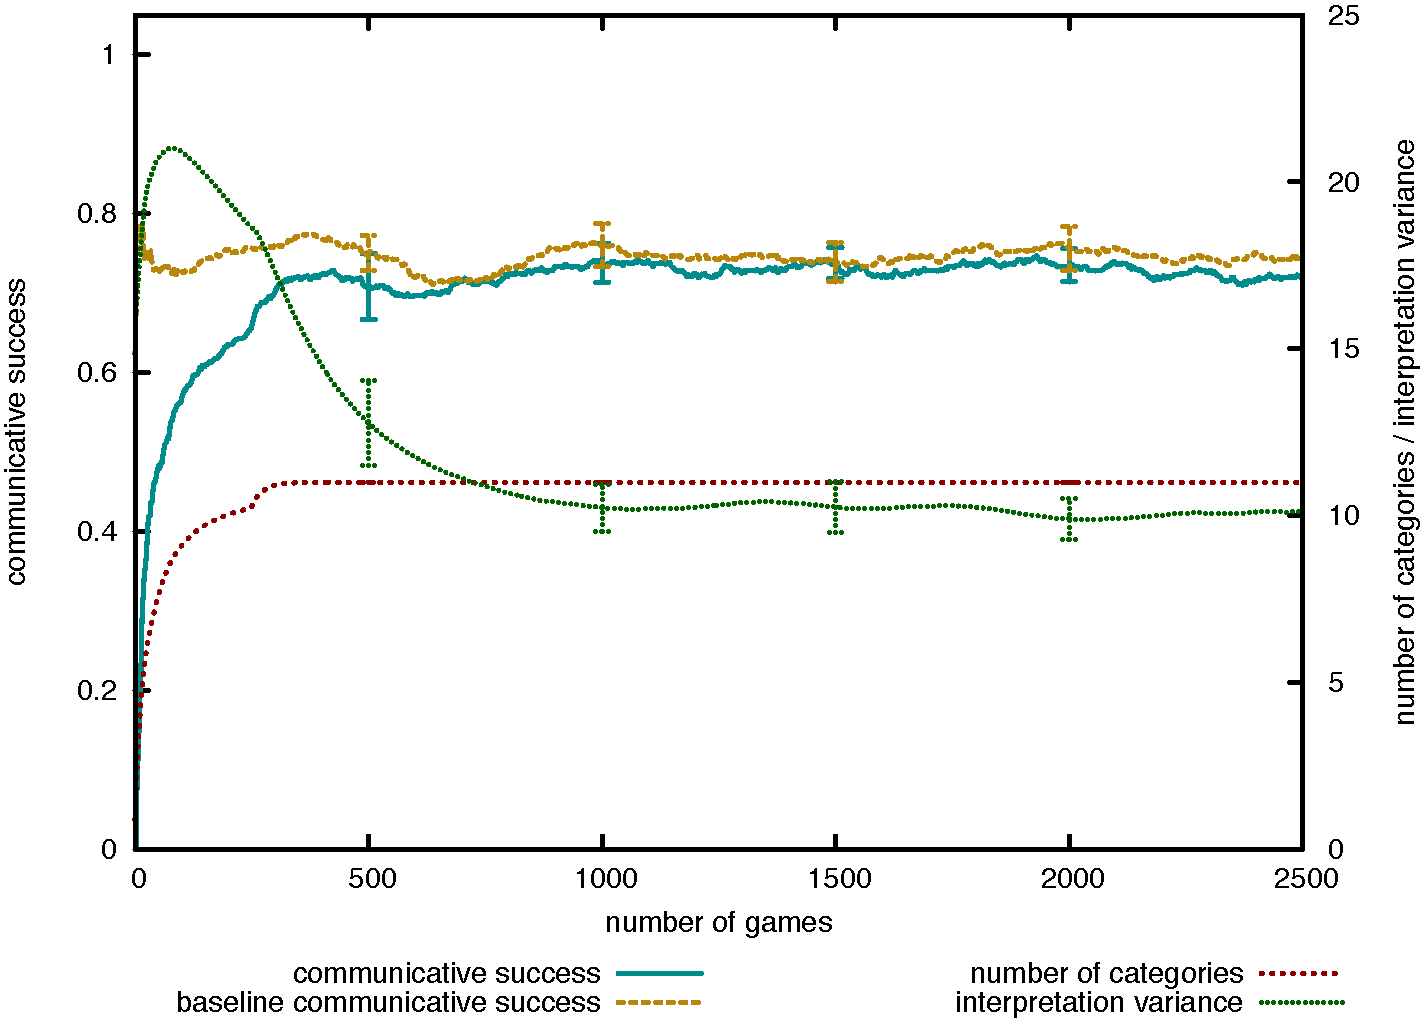
\includegraphics[width=.8\textwidth]{./basic-operators/figures/acquisition.pdf}
    \caption[Dynamics of an example acquisition experiment]{Dynamics
      of an example acquisition experiment in which the learner picks
      up a colour category system of the teacher. After 500
      interactions, the communicative success of the teacher-learner
      interactions is almost as high as in the baseline
      experiment. The interpretation variance decreases to a value of
      around 10.}
    \label{f:basic-strategy-agent-categories}
  \end{center}
\end{figure}

The interpretation variance never drops to zero, which reflects the
fact that the prototypes of the learned colour categories never
completely match the prototypes of the colour categories of the
teacher. The learner tries to position the prototype of each category
on the centroid of a term -- the most central colour of all the colours that will
be named by the teacher using the same term. Hence, the nonzero
interpretation variance can be explained if the prototypes used by the
teacher are not exactly at the centre of all colour samples that
belong to the same category. One possible explanation could be that
my model uses a different colour space than the one in which the
centroids were reported and computed in literature. \cite{sturges95location}
report their centroids in Munsell Colour System, 
whereas in my model the CIE $L^*a^*b^*$ colour space is used. 
As the transformation between these two spaces is not linear 
(see Appendix \ref{s:lab} and \ref{s:munsell}) a discrepancy between the prototypes 
of the teacher and the prototypes of the learner is to be expected.

The impact of the alignment rate on the interpretation variance is
explored in \figref{f:basic-strategy-alignment-rate-vs-variance}. It shows a
trade-off between accuracy and speed of learning. A learner agent that
uses a low alignment rate, will align more slowly but will end up
with a category system that more accurately represents the system of
the teacher. The variance of agents that do not align their categories
remains high.

\begin{figure}[htbp]
  \begin{center}
    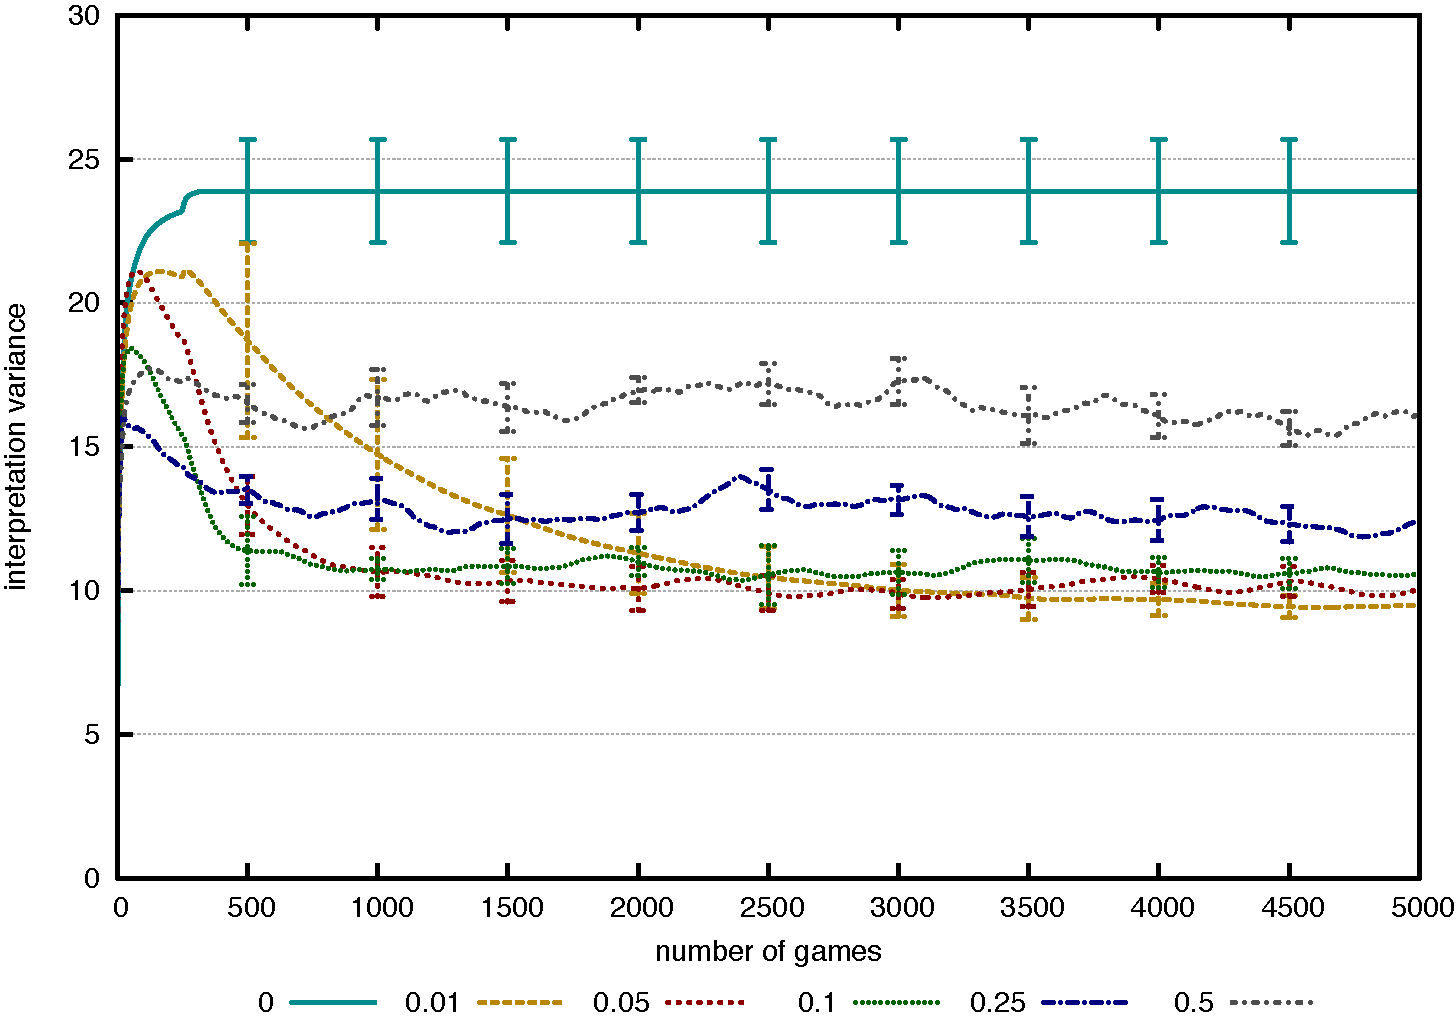
\includegraphics[width=.8\textwidth]{./basic-operators/figures/alignment-rate-vs-variance.pdf}
    \caption[Parameter study for alignment rate]{Parameter study for
      the alignment rate in relation to the interpretation variance
      between the resulting category system and the predefined
      language system. Higher alignment rates will result in faster
      but less accurate alignment.}
    \label{f:basic-strategy-alignment-rate-vs-variance}
  \end{center}
\end{figure}

\figref{f:basic-strategy-acquisition-lexicon} shows an example
acquisition process of a colour category system next to the target
colour system. After 100 interactions, the learning agent has already
learned the 11 different colour terms, but the prototypes of the
corresponding categories do not yet fully resemble the target colour
system. At the end of the acquisition experiment, the alignment of the
colour system is better.

\begin{figure}[htbp]
\centering
\subfigure[]{
  
\includegraphics[width=\textwidth]{./basic-operators/figures/acquisition-acquired-lexicon-100.pdf}
  \label{f:acquisition-acquired-lexicon-100}
}
\subfigure[]{
  
\includegraphics[width=\textwidth]{./basic-operators/figures/acquisition-acquired-lexicon-2500.pdf}
  \label{f:acquisition-acquired-lexicon}
}
\subfigure[]{
  
\includegraphics[width=\textwidth]{./basic-operators/figures/acquisition-target-lexicon.pdf}
  \label{f:acquisition-target-lexicon}
}
\caption[Example of an acquired and target colour system]{Example of
  acquired colour system: after 100 interactions
  \subref{f:acquisition-acquired-lexicon-100} and after 2500
  interactions \subref{f:acquisition-acquired-lexicon}. The target
  colour system is shown for comparison
  \subref{f:acquisition-target-lexicon}.}
\label{f:basic-strategy-acquisition-lexicon}
\end{figure}

\section{Invention operator}
\label{s:bcs-invention-operators}

The invention operator
\is{learning operators!invention operator!for basic colour strategy}
is triggered on the basis of not being able
to discriminate the randomly selected topic colour sample in a
context. Whenever this occurs, an agent might invent a new colour
category focussed on the current topic to which a newly invented form
will be associated. This form will be used to express this category in
language.

The rate at which new categories are invented is controlled by the
\textsc{colour category invention rate}
\is{invention rate!colour category}
\is{colour category invention rate|see{invention rate}}
parameter. If it is set to a low value, it ensures that categories get
a chance to spread into the population before another category gets
invented. In the reported experiments, this rate is constant and set
to 0.005.

Previous models \citep{steels05coordinating, belpaeme05explaining,
  belpaeme07language} did not use an invention rate, but instead implemented
mechanisms in which several terms could compete to express the same
colour category. This competition was coordinated using a lateral
inhibition scheme, which decreased the chances of competing terms being used
whenever a successful interaction took place. It has been shown that
such a mechanism leads to a one on one mapping between terms and
colour categories. Typically, these models also included the
functionality to merge two colour categories into one whenever they
became too similar to each other. 

The proposed use of an invention rate does not have a significant
impact on the reported results and could be thought of as a
simplification of previous models.

\subsection{Formation experiment}
\label{s:formation-experiment}
\is{formation experiment!for basic colour strategy}

In the formation experiment, a population of agents needs to form
their own colour category system from scratch. One context will
consist of three randomly chosen Munsell chips \citep{newhall42final},
but with the additional constraints of a minimal
interstimulus distance of 50 in the CIE $L^*u^*v^*$ colour space and
the reproducibility of colour categories in the Adobe 1998 RGB
colour system. Other environments display similar dynamics, but
require more colour categories and more time to align. The population
size is 10.

\subsection{Results}

\subsubsection{Brightness and hue strategy}

The resulting dynamics of the \textsc{brightness and hue strategy}, in
which all three dimensions of the colour space are used, are shown in
\figref{f:formation-full-dynamics}. The proposed strategy is
sufficient to allow a population of agents to form and align their own
colour category system. As in the acquisition experiment, the
interpretation variance decreases over time but has not stabilised
yet. The communicative success even surpasses the baseline
communicative success (which is estimated in \figref{f:bcs-baseline} to be just below 90\%). This however comes at the
cost of a few more colour categories than in the baseline which
consisted of 11 categories. As the adoption operator is implemented to
not consider synonymy, the number of categories (shown in ontology
size) is equal to the number of lexical entries in the lexicon (shown
in lexicon size).

\begin{figure}[htpb]
  \begin{center}
    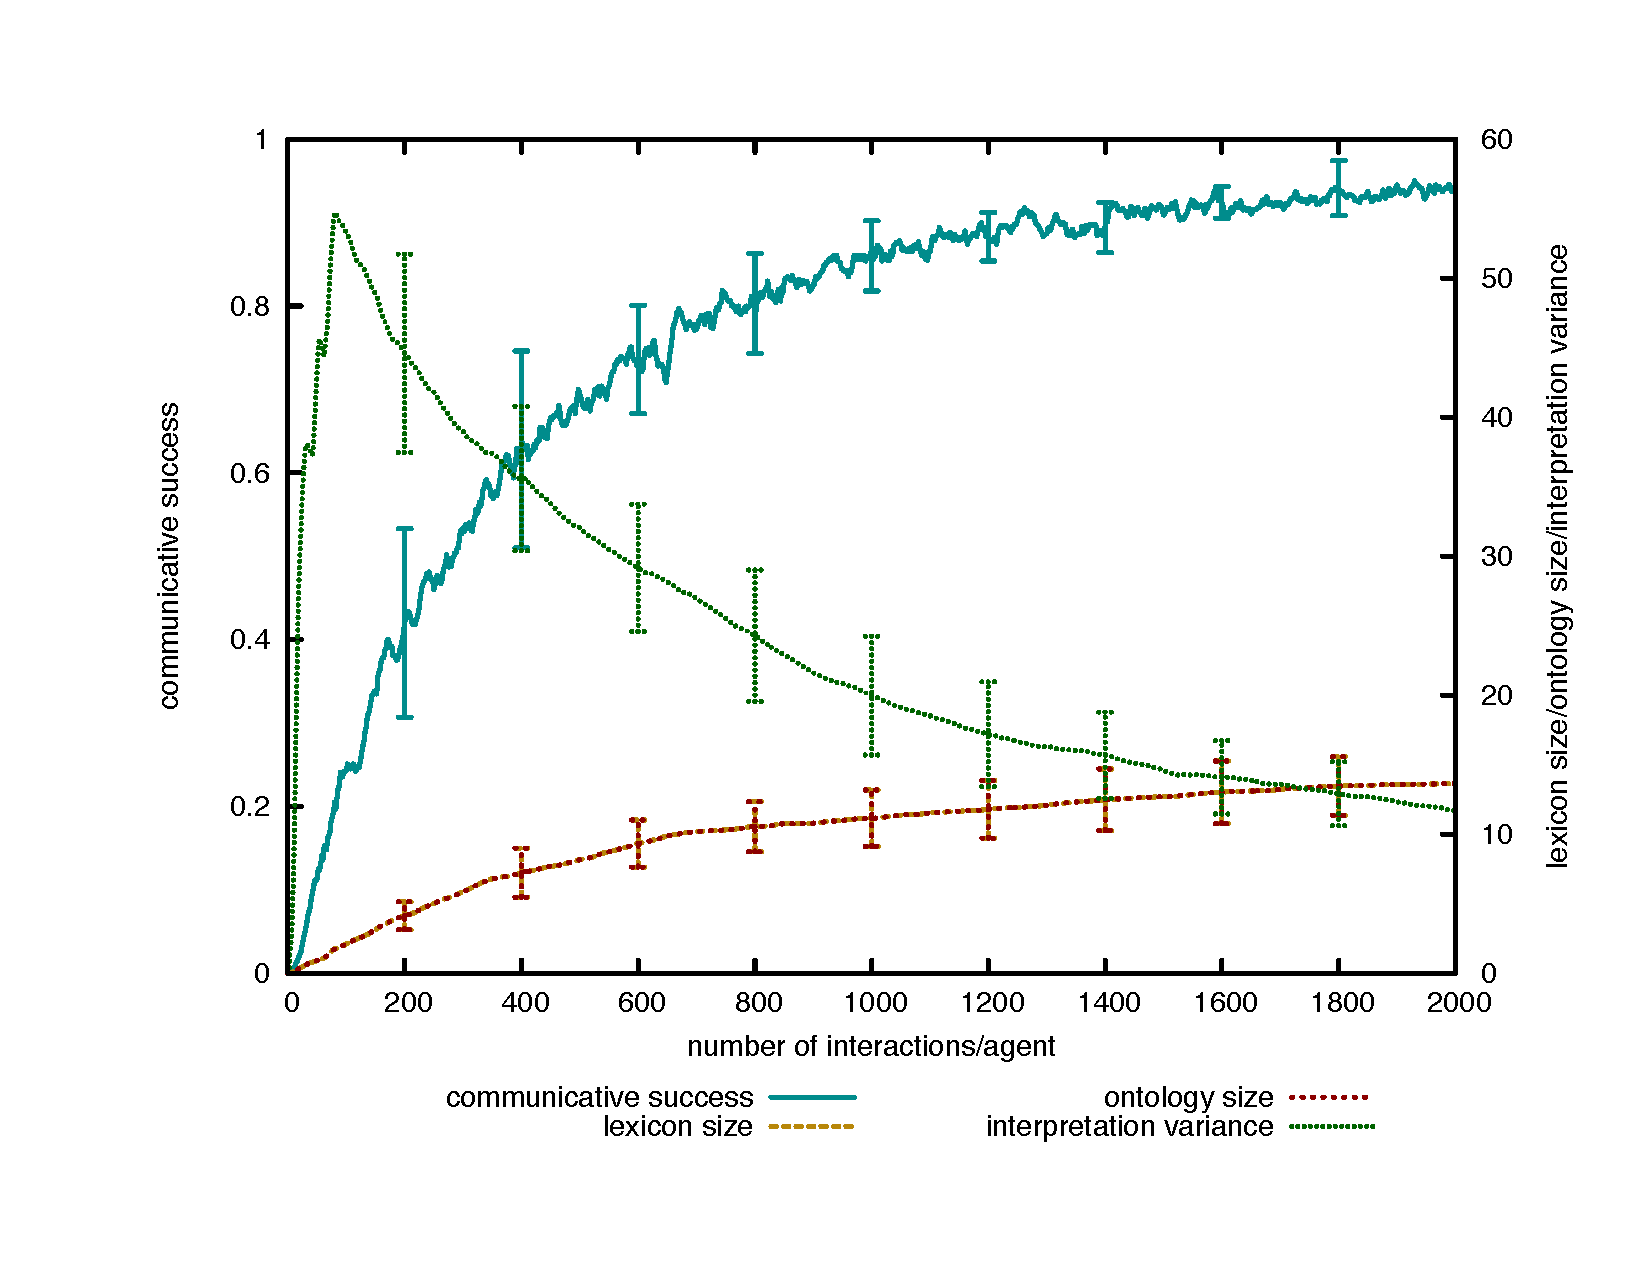
\includegraphics[width=0.8\textwidth]{./basic-operators/figures/formation-full.pdf}
    \caption[Dynamics of the formation experiment for the brightness
    and hue strategy]{Dynamics of the formation experiment for the
      brightness and hue strategy. The agents are able to coordinate a
      colour category system that is successful in the communicative
      environment.}
    \label{f:formation-full-dynamics}
  \end{center}
\end{figure}

An example of the self-organisation of a colour category system in a
population of 5 agents is shown in \figref{f:formation-full-lexicon}. Initially, a lot of variability
between the colour categories exists but this variability decreases
over time due to the alignment operator. The final colour system is
sufficiently coordinated to support successful communication.

\begin{figure}[htbp]
\centering
\subfigure[]{
  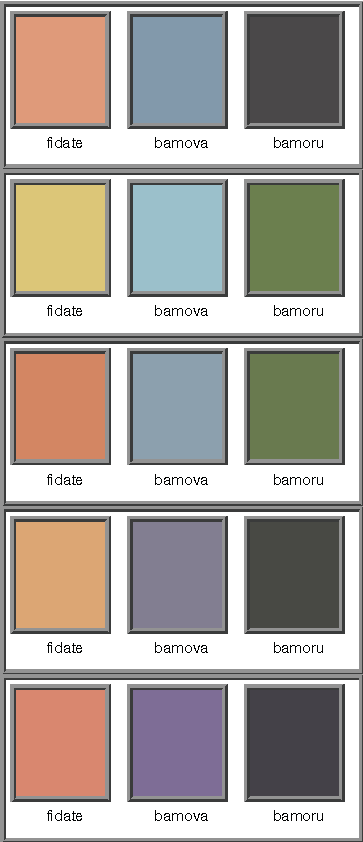
\includegraphics[height=5cm]{./basic-operators/figures/formation-full-lexicon-1000.pdf}
  \label{f:formation-full-lexicon-1000}
}
\subfigure[]{
  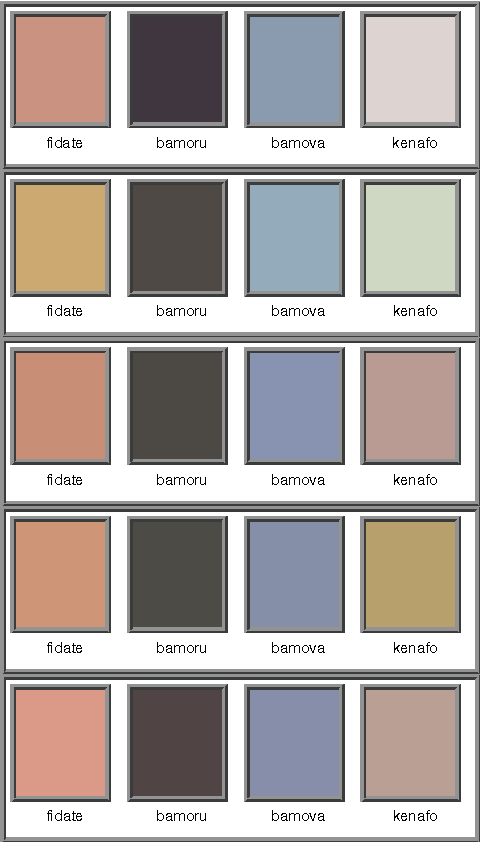
\includegraphics[height=5cm]{./basic-operators/figures/formation-full-lexicon-2000.pdf}
  \label{f:formation-full-lexicon-2000}
}
\subfigure[]{
  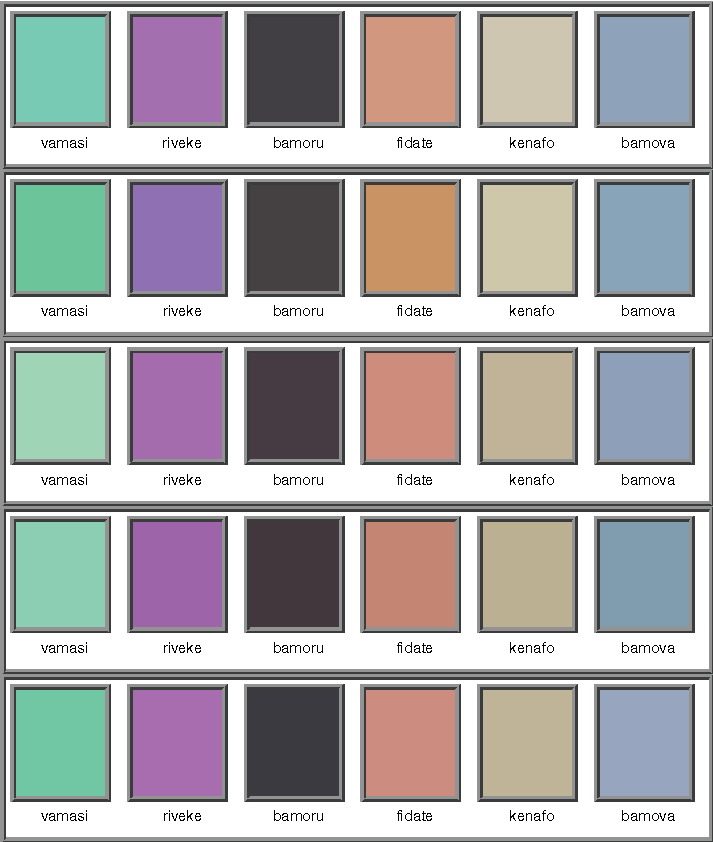
\includegraphics[height=5cm]{./basic-operators/figures/formation-full-lexicon-3000.pdf}
  \label{f:formation-full-lexicon-3000}
}
\caption[An evolving colour system for the basic colour strategy]{An
  evolving colour system for the basic colour strategy of a
  population of five agents after 200
  \subref{f:formation-full-lexicon-1000}, 400
  \subref{f:formation-full-lexicon-2000} and 600
  \subref{f:formation-full-lexicon-3000} interactions per agent. Each
  row shows the lexicon of one agent and the columns show the
  prototypes associated with a shared form.}
\label{f:formation-full-lexicon}
\end{figure}

\subsubsection{Brightness strategy}

The \textsc{brightness strategy}, in which only the brightness dimension
is profiled, is equally suitable to form a category system that is
adequate for the communicative challenge posed by the environment as
shown in \figref{f:formation-brightness-dynamics}, although a
slightly higher number of categories is required to achieve a slightly
lower communicative success. The main difference is that the invented
colour categories now do not possess any hue information and hence the
colour categories are shades of grey, as illustrated in \figref{f:formation-brightness-lexicon}.

\begin{figure}[p]
  \begin{center}
    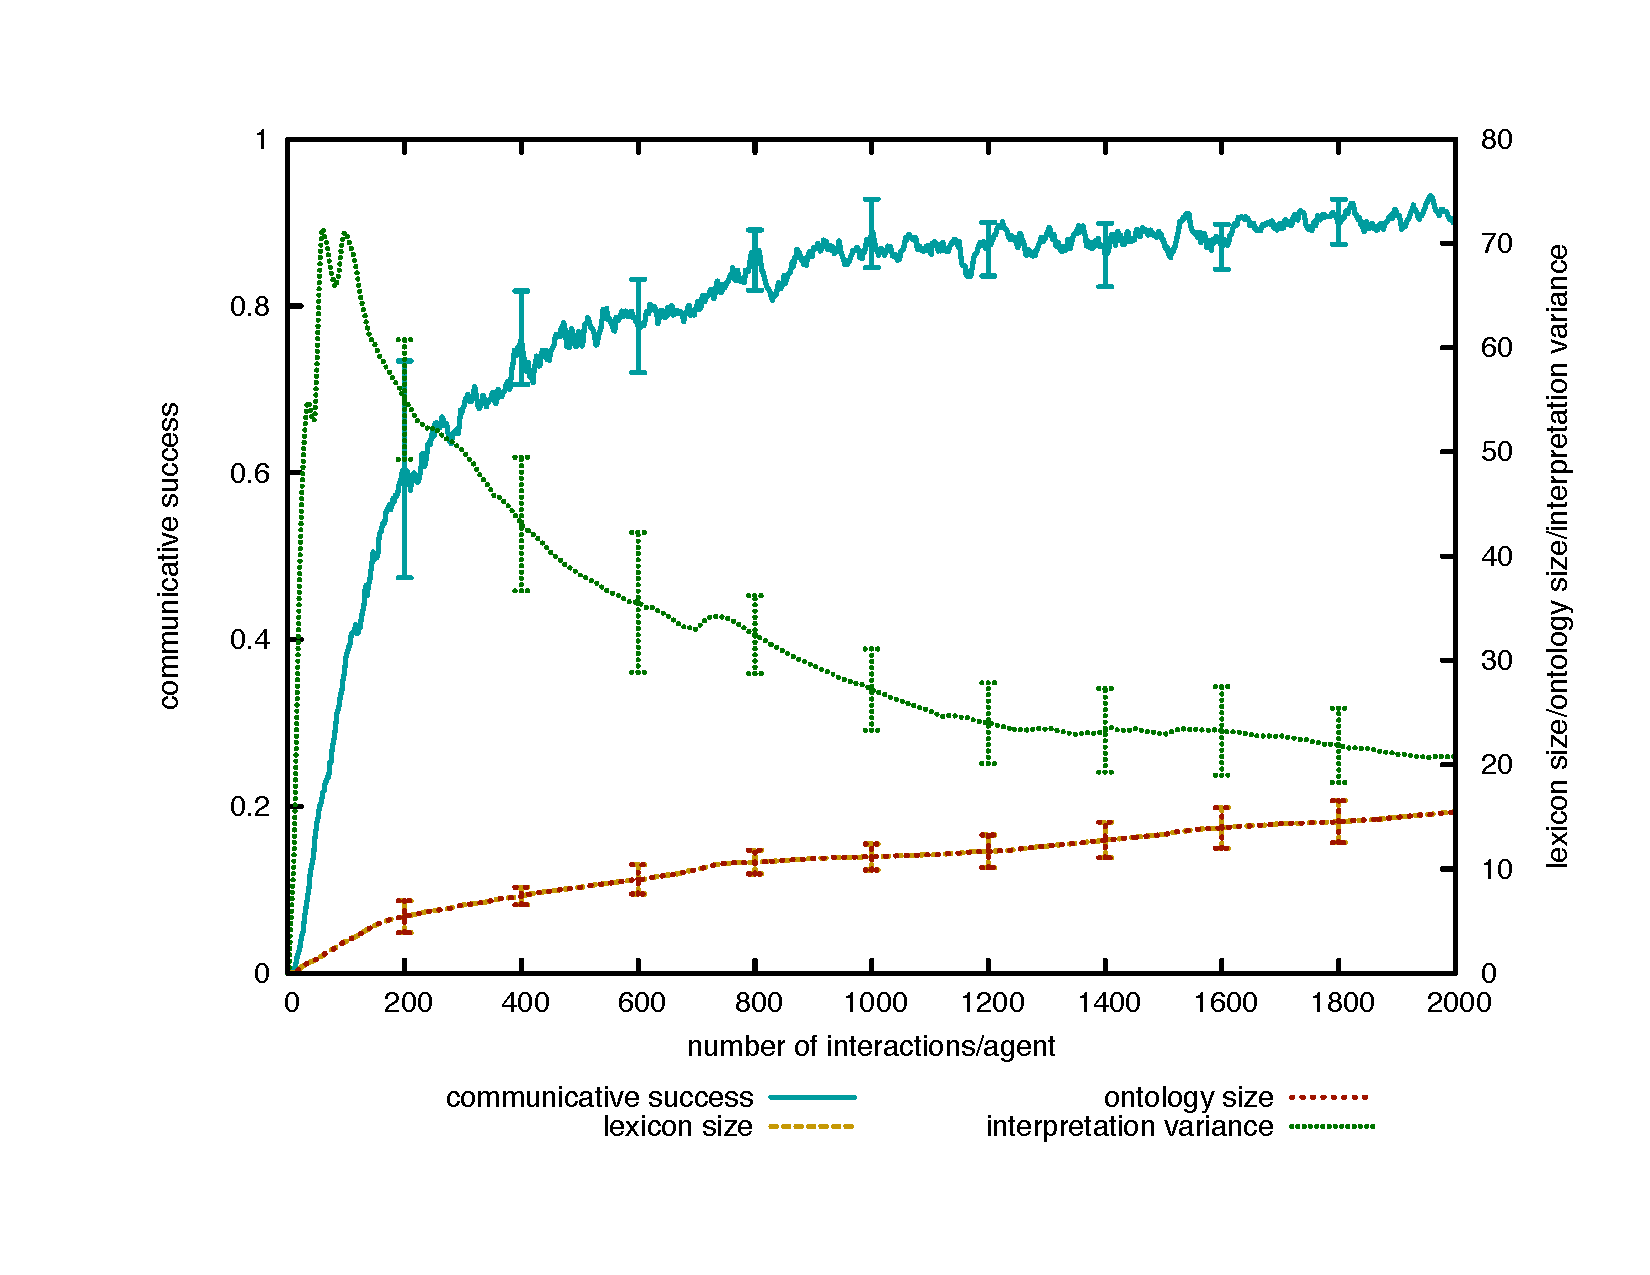
\includegraphics[width=0.8\textwidth]{./basic-operators/figures/formation-brightness.pdf}
    \caption[Dynamics of the formation experiment for the brightness
    strategy]{Dynamics of the formation experiment for the brightness
      strategy. The agents are able to coordinate a colour category
      system that is successful in the communicative environment.}
    \label{f:formation-brightness-dynamics}
  \end{center}
\end{figure}

\begin{figure}[p]
\centering
\subfigure[]{
  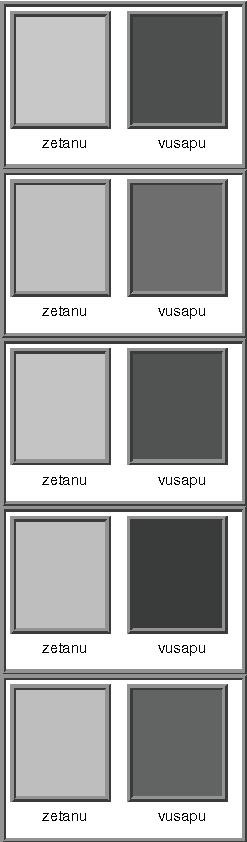
\includegraphics[height=5cm]{./basic-operators/figures/formation-brightness-lexicon-1000.pdf}
  \label{f:formation-brightness-lexicon-1000}
}
\subfigure[]{
  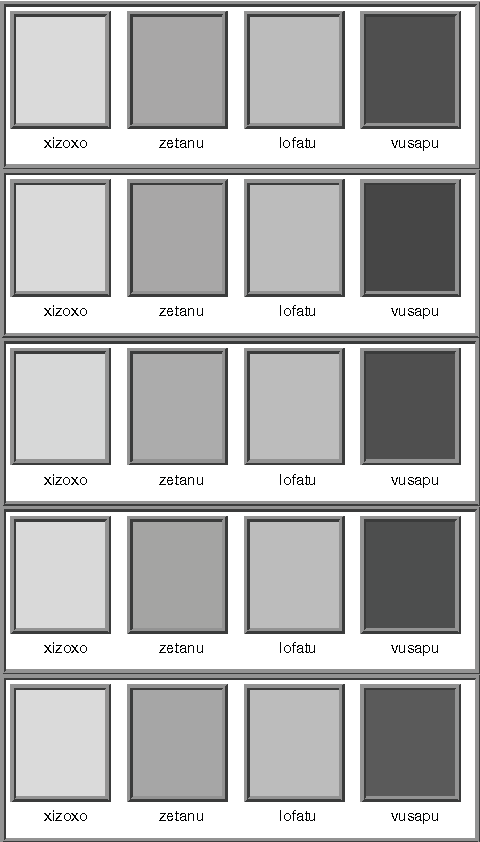
\includegraphics[height=5cm]{./basic-operators/figures/formation-brightness-lexicon-3000.pdf}
  \label{f:formation-brightness-lexicon-3000}
}
\subfigure[]{
  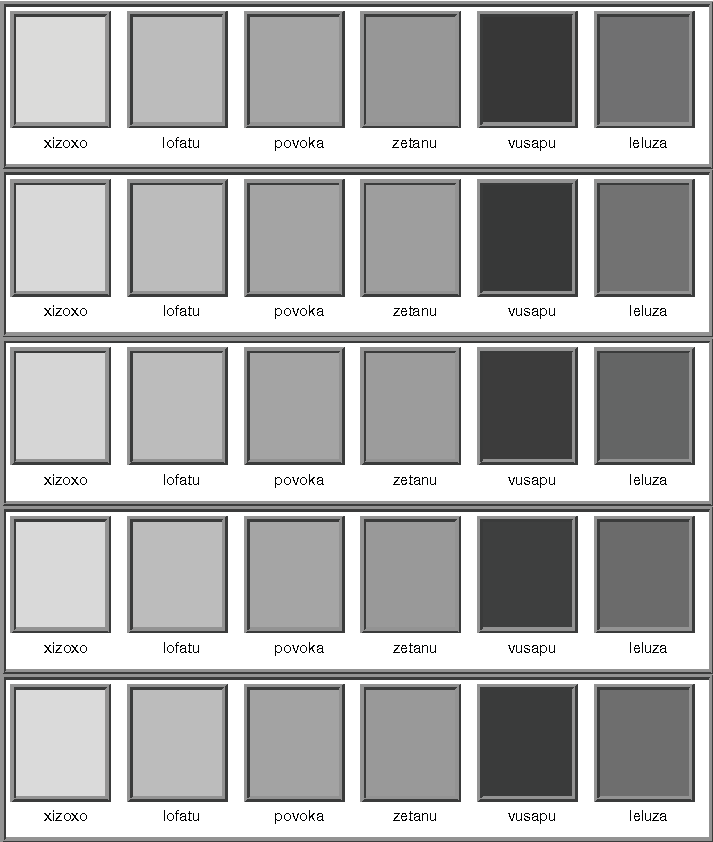
\includegraphics[height=5cm]{./basic-operators/figures/formation-brightness-lexicon-4000.pdf}
  \label{f:formation-brightness-lexicon-4000}
}
\caption[An evolving colour system for the brightness strategy]{An
  evolving colour system for the brightness strategy of a population
  of five agents after 200
  \subref{f:formation-brightness-lexicon-1000}, 600
  \subref{f:formation-brightness-lexicon-3000} and 800
  \subref{f:formation-brightness-lexicon-4000} interactions per
  agent. Each row shows the lexicon of one agent and the columns show
  the prototypes associated with a shared form.}
\label{f:formation-brightness-lexicon}
\end{figure}
\clearpage

\section{Conclusion}

By specifying the acquisition and invention operators of a language
strategy, it becomes possible to study the self-organisation of a language
system based on that language strategy. The acquisition operators
allow simulated agents to acquire a basic colour language system from
one another and invention operators that allow a population of agents
to invent their own language system. The performance of the
acquisition operator can be evaluated by comparing the communicative
success of an agent that acquires a predefined language from another
agent. In a formation experiment, a population of agents need to
invent a language system from scratch. This experiment allows to check
the performance of the invention operators.

\newpage
\thispagestyle{empty}
